\section{Testing}
\subsection{Unit Testing}
Each VHDL submodule we implemented has its own testbench created by us.
We tried following test-driven development practices by writing failing tests first, then implementing the feature(s) to make the tests pass.
Tests were written based on our assumptions and since we lack experience,
sometimes needed to be changed as we learned more and corrected our implementation.

\subsection{System Testing}
\subsubsection{tb\_MIPSProcessor}
A testbench for the processor was provided.
This loads data and instruction to the memories,
lets the processor run for a while,
then checks that the data memory contains what it expects.
Our processor implementation passes all the tests of this testbench.

\subsubsection{On the FPGA}
After passing all the tests of \texttt{tb\_MIPSProcessor},
we adapted the same program to make it compatible with the HostComm tool,
then synthesized and created a bitfile of the whole MIPSSystem.

\begin{figure}[h]
    \centering
    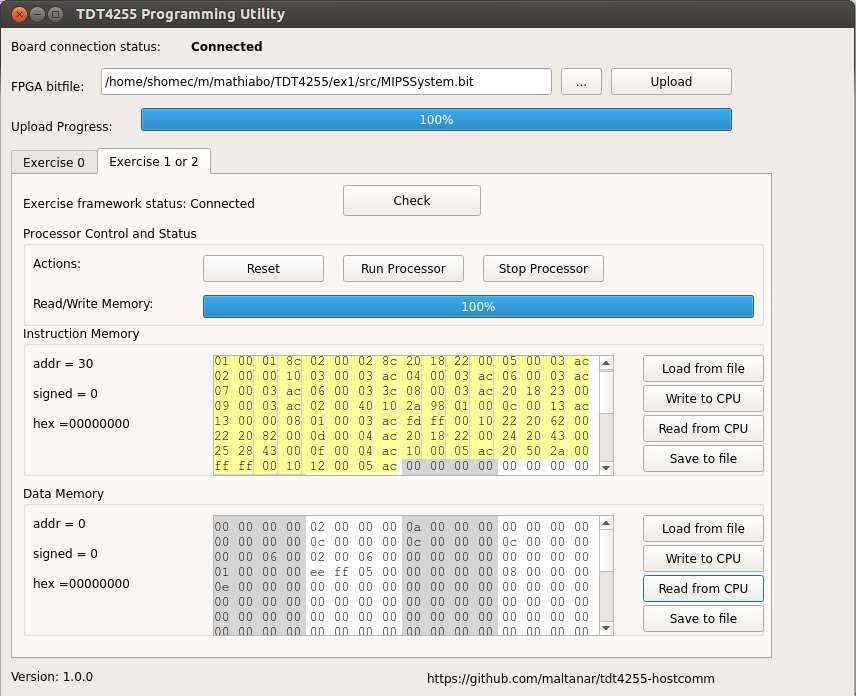
\includegraphics[width=\textwidth]{img/Hostcomm}
    \caption{HostComm after running the processor on the FPGA. The values in the data memory has been read from CPU.}
    \label{fig:hostcomm}
\end{figure}
